\chapter{Limits: Approaching Values}

\section{Beginning Limits}

\subsection{Introduction}

The concept of a limit is based around what happens to a function as its input approaches, but not necessarily equals a certain value. This is an important concept in calculus and forms the mathematical basis for both derivatives and integrals later on.

For some intuition, we will look at a few examples.

\begin{example}{approaching values}
    Let us take a look at the function \( y = x^2 \). It is clear that the function is defined for all \( x \) values.
    
    \begin{center}
    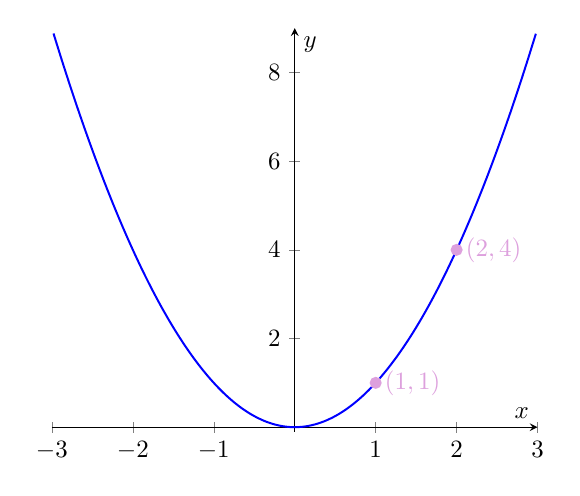
\begin{tikzpicture}[scale=0.9]
        \begin{axis}[xmin=-3, xmax=3, xstep=1, ymin=-0.1, ymax=9, ystep=1, axis lines=middle, xlabel=\(x\), ylabel=\(y\), restrict y to domain=-0.1:9, clip=false, every axis plot/.append style={thick}]
            \addplot[color=blue, samples=100, smooth]{x^2};
            \addplot[color=Plum,mark=*] coordinates {(1,1)} node[right, pos=1]{\( (1, 1) \)};
            \addplot[color=Plum,mark=*] coordinates {(2,4)} node[right, pos=1]{\( (2, 4) \)};
        \end{axis}
    \end{tikzpicture}
    \end{center}
    
    After reading the graph, it should be clear that, as \( x \) approaches \( 1 \) from both the left and right sides, \( y \) approaches \( 1 \) as well. Similarly, as \( x \) approaches \( 2 \), \( y \) approaches \( 4 \). One could also say that when \( x = 1 \), \( y = 1 \), or when \( x = 2 \), \( y = 4 \), and they would be right; however, the value of the function at a point (as we'll come to see) will not always be the exact same value as when \( x \) approaches that point.
\end{example}

\begin{example}{approaching values}
    Consider the function \( f \left( x \right) = \frac{x - 1}{x - 1} \). While algebraically we can simplify this to \( y = 1 \), we do see that there is a restriction that \( x \ne 1 \), leaving us with an unpleasant "hole" in the graph. Despite this, we can say that the function "looks" to be approaching the value \( 1 \) as \( x \) gets closer and closer to the value \( 1 \).
    
    \begin{center}
    \begin{tikzpicture}[scale=0.9]
        \begin{axis}[xmin=-2, xmax=2, xstep=1, ymin=-2, ymax=2, ystep=1, axis lines=middle, xlabel=\(x\), ylabel=\(y\), every axis plot/.append style={thick}]
            \addplot[color=blue]{1} node {\( f \left( x \right) \)};
            \addplot[hole, color=blue, fill=examplebg] coordinates{(1, 1)};
        \end{axis}
    \end{tikzpicture}
    \end{center}
\end{example}

Using this intuition of "approaching," we can form our understanding of what a limit actually is.

\begin{definition}{limit}
    Given \( c, L \in \mathbb{R} \), if the values of some function \( f \left( x \right) \) approach or equal \( L \) as the values of \( x \) approach, but do not necessarily equal, \( c \), we say that the function \( f \) has the \defterm{limit} \( L \) as \( x \) approaches \( c \).
    
    \vspace{0.3cm}
    
    Note that, in order for a limit to exist, the function should approach a single value (remember \( \infty \) is not a value), and the function should approach that value from both sides. Limits are unique, so there will never be multiple values for a limit.
\end{definition}

\begin{notation}{limit}
    The correct way to write a limit is as follows,
    
    \[ \lim_{x \to c} f \left( x \right) = L \]
    
    We can read this as "the limit of \( f \) of \( x \) as \( x \) approaches \( c \) equals \( L \)."
    
    When a limit does not exist at a point, we write "DNE" (does not exist) to indicate so.
\end{notation}

\subsection{Evaluating Limits}

A limit can be thought of as a command, telling a mathematician to find the value that the expression "should" equal. Some limits will be simplified through simple substitution, while others will require more intensive algebra. Take a simple example first.

\begin{example}{limit substitution}
    Find
    
    \[ \lim_{x \to 2} \left( x + 2 \right) \]
    
    Simply substituting the value \( x = 2 \) into the limit, we can easily arrive at our answer.
    
    \begin{align}
        & \lim_{x \to 2} \left( x + 2 \right) \\
        = \> &\left( 2 + 2 \right) \\
        = \> &4
    \end{align}
\end{example}

Under the scope of limits, we can also evaluate functions that would otherwise have restrictions. Limits allow us to forgo rules like division by \( 0 \), so long as the algebra allows it. To understand what this means, let us take a look at another example.

\begin{example}{indeterminate form}
    Find
    
    \[ \lim_{x \to 2} \dfrac{x - 2}{x - 2} \]
    
    For this example, just substituting \( x = 2 \) into the limit will not work, giving us \( \frac{0}{0} \), a type of \defterm{indeterminate form}. Here, then, we must use algebra to simplify the limit.
    
    \begin{align}
        &\lim_{x \to 2} \dfrac{x - 2}{x - 2} \\
        = \> &\lim_{x \to 2} \dfrac{\cancel{x - 2}}{\cancel{x - 2}} \\
        = \> &1
    \end{align}
\end{example}

\begin{tip}
    In the previous example, there are two very important details to notice.
    
    \begin{enumerate}
        \item Until you have eliminated all limit variables, the limit symbol \textbf{must} stay in the expression.
        \item Once you have crossed off a limit variable, that limit \textbf{must} disappear, and the steps following should be your final answer, not containing any further mention to that variable.
    \end{enumerate}
\end{tip}

\begin{definition}{indeterminate form}
    A term you may have noticed used in the previous example is \defterm{indeterminate form}. An indeterminate form is a consequence of the workings of limits and is found when evaluating certain expressions. There are several types indeterminate forms, as seen here.
    
    \begin{multicols}{3}
    \begin{itemize}
        \item \( \dfrac{0}{0} \)
        \item \( \dfrac{\infty}{\infty} \)
        \item \( 0 \cdot \infty \)
        \item \( \infty - \infty \)
        \item \( 0^0 \)
        \item \( 1^\infty \)
        \item \( \infty^0 \)
    \end{itemize}
    \end{multicols}
    
    The appearance of an indeterminate form does not signal that the limit exists nor does not exist. Also note that the value of an indeterminate limit can take on any value. Do \textbf{\color{tipfg}not} be fooled into thinking that
    
    \[ \dfrac{0}{0} = 1 \]
    
    will always be true. In the first place, do not use the \( = \) symbol when not dealing with defined numbers.
\end{definition}

For further clarification, here is another example.

\begin{example}{evaluating limits}
    Find
    
    \[ \lim_{x \to 0} \dfrac{\left( x + 3 \right)^2 - 9}{x} \]
    
    Once again, a simple substitution will result in a \( \frac{0}{0} \) indeterminate form, so let us try to simplify the expression using algebra in order to see if the limit exists.
    
    \begin{align}
        &\lim_{x \to 0} \dfrac{\left( x + 3 \right)^2 - 9}{x} \\
        = \> &\lim_{x \to 0} \dfrac{x^2 + 6x + 9 - 9}{x} \\
        = \> &\lim_{x \to 0} \dfrac{x^{\cancel{2}} + 6\cancel{x}}{\cancel{x}} \\
        = \> &6
    \end{align}
\end{example}

In particular, many limits will also utilize sums or differences of squares and cubes, which you should be on the lookout for to see if you can cancel something in the numerator and denominator. Another generally helpful rule is to always reduce fractions and cancel terms before attempting other simplifications.

\subsection{Limits with Tables}

Although not as common, you can evaluate a limit by creating a table of values, with \( x \) approaching the desired value from both sides.

\begin{example}{finding limits with tables}
    Suppose you are asked to evaluate
    
    \[ \lim_{x \to 2} \left( x - 4 \right) \]
    
    While substituting in the value would work, sometimes you will be asked to find the limit using tables. It is also important to be able to read tables if you are asked to find the limits from them.
    
    For this limit, we can make two tables, with \( x \) approaching \( 2 \) from the left side and then from the right side.
    
    \begin{center}
    \begin{tabular}{c|c}
        \( x \) & \( x - 4 \) \\
        \hline
        \( 1.9 \)     & \( -2.1 \) \\
        \( 1.99 \)    & \( -2.01 \) \\
        \( 1.999 \)   & \( -2.001 \) \\
        \( 1.9999 \)  & \( -2.0001 \) \\
        \( 1.99999 \) & \( -2.00001 \) \\
    \end{tabular}
    \hspace{0.5cm}
    \begin{tabular}{c|c}
        \( x \) & \( x - 4 \) \\
        \hline
        \( 2.1 \)     & \( -1.9 \) \\
        \( 2.01 \)    & \( -1.99 \) \\
        \( 2.001 \)   & \( -1.999 \) \\
        \( 2.0001 \)  & \( -1.9999 \) \\
        \( 2.00001 \) & \( -1.99999 \) \\
    \end{tabular}
    \end{center}
    
    From looking at the tables, we can see that the limit approaches \( -2 \) from both sides.
\end{example}

\subsection{Limit Properties and Rules}

There are certain properties and rules that limits abide by that can aid in evaluating them.

\begin{theorem}{Theorem}
    If \( f \left( x \right) = k \), where \( k \) is a constant, then for all \( c \in \mathbb{R} \),
    
    \[ \lim_{x \to c} f \left( x \right) = \lim_{x \to c} \left( k \right) = k \]
    
    Essentially, the theorem above states that for some constant function, the limit for any point of that function will be the constant.
\end{theorem}

\begin{example}{limit of a constant}
    Suppose that \( f \left( x \right) = 2 \). Then
    
    \begin{align}
        &\lim_{x \to 10} f \left( x \right) = 2 \\
        = \> &\lim_{x \to 10} y = 2 \\
        = \> &\lim_{x \to 10} 2 = 2
    \end{align}
\end{example}

Limits also have specific rules that allow them to be combined and manipulated in certain ways.

For all \( L_1, L_2 \in \mathbb{R} \), if \( \lim_{x \to c} f \left( x \right) = L_1 \) and \( \lim_{x \to c} g \left( x \right) = L_2 \) then,

\begin{definition}{Sum Rule}
    \[ \lim_{x \to c} \left( f \left( x \right) + g \left( x \right) \right) = L_1 + L_2 \]
\end{definition}

\begin{example}{Sum Rule}
    \begin{align}
        &\left( \lim_{x \to 2} x^2 \right) + \left( \lim_{x \to 2} x \right) \\
        = \> &\lim_{x \to 2} \left(x^2 + x \right) \\
        = \> &\left( 2 \right)^2 + \left( 2 \right) \\
        = \> &6
    \end{align}
\end{example}

\begin{definition}{Difference Rule}
    \[ \lim_{x \to c} \left( f \left( x \right) - g \left( x \right) \right) = L_1 - L_2 \]
\end{definition}

\begin{example}{Difference Rule}
    \begin{align}
        &\left( \lim_{x \to 2} 3x \right) - \left( \lim_{x \to 2} 2 \right) \\
        = \> &\lim_{x \to 2} \left(3x - 2 \right) \\
        = \> &3\left( 2 \right) - 2 \\
        = \> &4
    \end{align}
\end{example}

\begin{definition}{Constant Multiple Rule}
    \[ \lim_{x \to c} k f \left( x \right) = k L_1 \]
\end{definition}

\begin{example}{Constant Multiple Rule}
    \begin{align}
        &3 \left( \lim_{x \to 5} 2x^2 \right) \\
        = \> &\lim_{x \to 5} 6x^2 \\
        = \> &6 \left( 5 \right)^2 \\
        = \> &750
    \end{align}
\end{example}

\begin{definition}{Product Rule}
    \[ \lim_{x \to c} \left( f \left( x \right) g \left( x \right) \right) = L_1 L_2 \]
\end{definition}

\begin{example}{Product Rule}
    \begin{align}
        &\left( \lim_{x \to 3} x \right)^2 \\
        = \> &\left( \lim_{x \to 3} x \right) \left( \lim_{x \to 3} x \right) \\
        = \> &\lim_{x \to 3} x^2 \\
        = \> &9
    \end{align}
\end{example}

\begin{definition}{Quotient Rule}
    \[ \lim_{x \to c} \dfrac{f \left( x \right)}{g \left( x \right)} = \dfrac{L_1}{L_2}, \quad L_2 \ne 0 \]
\end{definition}

\begin{example}{Quotient Rule}
    \begin{align}
        &\dfrac{1}{\left( \lim_{x \to 0} \dfrac{1}{x} \right)} \\
        = \> &\lim_{x \to 0} x \\
        = \> &0
    \end{align}
\end{example}

\subsection{Limits with Graphs}

Consider the function \( y = \lfloor x \rfloor \).

\begin{center}
\begin{tikzpicture}
    \begin{axis}[xmin=-5, xmax=5, xstep=1, ymin=-5, ymax=5, ystep=1, axis lines=middle, xlabel=\(x\), ylabel=\(y\), every axis plot/.append style={very thick}]
        \addplot[color=blue, jump mark mid, samples=50, domain=-4:4]{floor(x)};
        \addplot[color=blue,mark=*] coordinates {(-4,-4)};
        \addplot[color=blue,mark=*] coordinates {(-3,-3)};
        \addplot[color=blue,mark=*] coordinates {(-2,-2)};
        \addplot[color=blue,mark=*] coordinates {(-1,-1)};
        \addplot[color=blue,mark=*] coordinates {(0,0)};
        \addplot[color=blue,mark=*] coordinates {(1,1)};
        \addplot[color=blue,mark=*] coordinates {(2,2)};
        \addplot[color=blue,mark=*] coordinates {(3,3)};
        
        \addplot[hole,color=blue,fill=bg] coordinates {(-3, -4)};
        \addplot[hole,color=blue,fill=bg] coordinates {(-2, -3)};
        \addplot[hole,color=blue,fill=bg] coordinates {(-1, -2)};
        \addplot[hole,color=blue,fill=bg] coordinates {(0, -1)};
        \addplot[hole,color=blue,fill=bg] coordinates {(1, 0)};
        \addplot[hole,color=blue,fill=bg] coordinates {(2, 1)};
        \addplot[hole,color=blue,fill=bg] coordinates {(3, 2)};
        \addplot[hole,color=blue,fill=bg] coordinates {(4, 3)};
    \end{axis}
\end{tikzpicture}
\end{center}

We can see that, for any non-integer value \( c \), the limit will be some integer. But what of at integer values? What if we approach from only one side?

\begin{notation}{Left and Right-Hand Limits}
    When taking one sided limits, we use a minus or plus sign in the exponent of the \( c \) value to denote which side we are approaching from.
    A minus sign indicates that we are approaching from the left, or negative, side.
    
    \[ \lim_{x \to c^-} f \left( x \right) \]
    
    A plus sign indicates that we are approaching form the right, or positive, side.
    
    \[ \lim_{x \to c^+} f \left( x \right) \]
    
    Remember that for the limit to exist, both sides of the limit must exist \textbf{and} be equal.
\end{notation}

\begin{example}{floor limits}
    Using the graph of the floor function from earlier, we can see that
    
    \[ \lim_{x \to 2^-} \lfloor x \rfloor = 1 \]
    
    Furthermore, we can also see that
    
    \[ \lim_{x \to 2^+} \lfloor x \rfloor = 2 \]
    
    This is similar for any integer, not just \( c = 2 \). Knowing that the floor function rounds down, these limit values should not come as a surprise.
    
    \vspace{0.3cm}
    
    Although both the left and right-sided limits exist, we can see that they are obviously not equal; therefore, we can say that
    
    \[ \lim_{x \to c} \lfloor x \rfloor \text{ DNE} \]
    
    for any integer value \( c \).
\end{example}

Another highly important graph and limit to know revolves around the function \( y = \dfrac{\sin{x}}{x} \).

\begin{center}
\begin{tikzpicture}
    \begin{axis}[
        xmin=-5.5 * pi,
        xmax=5.5 * pi,
        xtick={-5 * pi, -4 * pi, -3 * pi, -2 * pi, -pi, 0, pi, 2 * pi, 3 * pi, 4 * pi, 5 * pi},
        xticklabels={\( -5\pi \), \( -4\pi \), \( -3\pi \), \( -2\pi \), \( -\pi \), \( 0 \), \( \pi \), \( 2 \pi \), \( 3 \pi \), \( 4 \pi \), \( 5 \pi \)},
        xticklabel style={anchor=north}, 
        ymin=-1,
        ymax=1.25,
        axis lines=middle,
        xlabel=\(x\),
        ylabel=\(y\),
        every axis plot/.append style={thick}
    ]
        \addplot[color=blue, samples=200, domain=-5*pi:5*pi]{sin(deg(x)) / x};
        \addplot[hole, color=blue, fill=bg] coordinates{(0, 1)};
    \end{axis}
\end{tikzpicture}
\end{center}

By graphical verification (a more rigorous, geometric proof can be found involving the unit circle), we see the following limit

\[ \lim_{x \to 0} \dfrac{\sin{x}}{x} = 1 \]

holds true. This limit forms the basis of evaluating several other trigonometric limits.

\begin{example}{trigonometric limit}
    Find
    
    \[ \lim_{x \to 0} \dfrac{2 \sin{5x}}{7x} \]
    
    Using the properties of limits as well as the limit above, we find
    
    \begin{align}
        &\lim_{x \to 0} \dfrac{2 \sin{5x}}{7x} \\
        = \> &\dfrac{2}{7} \lim_{x \to 0} \dfrac{\sin{5x}}{x} \\
        = \> & 5 \cdot \dfrac{2}{7} \lim_{x \to 0} \dfrac{\sin{5x}}{5x} \\
        = \> & 5 \cdot \dfrac{2}{7} \cancelto{1}{\lim_{x \to 0} \dfrac{\sin{5x}}{5x}} \\
        = \> & \dfrac{10}{7}
    \end{align}
\end{example}

For more involved examples and identities, look at some of the problems found in the curve packet.

\vspace{0.5cm}

Another highly important detail to remember is the \defterm{Sandwich Theorem}, also called the Squeeze Theorem.

\begin{theorem}{The Sandwich Theorem}
    Suppose that \( g \left( x \right) \le f \left( x \right) \le h \left( x \right) \) for all \( x \ne c \) in some interval about \( c \) and that:
    
    \[ \lim_{x \to c} g \left( x \right) = \lim_{x \to c} h \left( x \right) = L \]
    
    Then
    
    \[ \lim_{x \to c} f \left( x \right) = L \]
\end{theorem}

\begin{tip}
    All named theorems given in class need to be memorized \textbf{word for word}. These theorems are fair game to be asked on any test throughout the year, either through application or simple reciting. Also, most answers involving the use of a theorem should also contain a sentence explaining the answer.
\end{tip}

\begin{example}{The Sandwich Theorem}
    Using the Sandwich Theorem, prove that
    
    \[ \lim_{x \to 0} x^2 \sin{\left( \dfrac{1}{x} \right)} = 0 \]
    
    Using the fact that \( -1 \le \sin{\left( x \right)} \le 1 \) for all real numbers \( x \),
    
    \begin{align}
        -1 \le \> &\sin{\left( \dfrac{1}{x} \right)} \le 1 \\
        -x^2 \le \> &x^2 \sin{\left( \dfrac{1}{x} \right)} \le x^2 \\
        \lim_{x \to 0} -x^2 \le \> &\lim_{x \to 0} x^2 \sin{\left( \dfrac{1}{x} \right)} \le \lim_{x \to 0} x^2 \\
        0 \le \> &\lim_{x \to 0} x^2 \sin{\left( \dfrac{1}{x} \right)} \le 0
    \end{align}
    
    Thus, as desired
    
    \[ \lim_{x \to 0} x^2 \sin{\left( \dfrac{1}{x} \right)} = 0 \]
    
    An example sentence for the justification of the procedure above could be:
    
    "I squeezed \( x^2 \sin{\left( \frac{1}{x} \right)} \) between \( -x^2 \) and \( x^2 \), and the limit of \( -x^2 \) as \( x \) approaches \( \infty \) is equal to the limit of \( x^2 \) as \( x \) approaches \( \infty \) is equal to \( 0 \); therefore, the limit of \( x^2 \sin{\left( \frac{1}{x} \right)} \) as \( x \) approaches \( \infty \) is \( 0 \)."
\end{example}

\section{Limits Involving Infinity}

This section tackles the question of what happens when \( x \) gets really big or really small.

\subsection{End Behavior and End Behavior Models}

Consider the function \( y = \frac{1}{x} \). What happens as \( x \) approaches both \( -\infty \) and \( \infty \)? Either through intuition or graphing, you should be able to see that

\[ \lim_{x \to \infty} y = 0 \]

and

\[ \lim_{x \to -\infty} y = 0 \]

We call this the \defterm{end behavior} of the function \( y = \frac{1}{x} \).

\begin{definition}{end behavior}
    The \defterm{end behavior} of the function is value(s) that the function approaches as \( x \) approaches \( \pm \infty \).
    
    \vspace{0.5cm}
    
    These values that the function approaches at the infinities are also the same as horizontal asymptotes. If the function goes up to \( \infty \) or down to \( -\infty \), then there is not a horizontal asymptote on that side.
\end{definition}

\begin{example}{end behavior}
    The end behavior of the function \( y = \frac{1}{x} \) is \( 0 \).
\end{example}

One important distinction to make is that of end behavior and the \defterm{end behavior model}.

\begin{definition}{end behavior model}
    The \defterm{end behavior model} of a function is a \textit{function} that models what the original function looks like as \( x \) approaches \( \pm\infty \).
\end{definition}

\begin{example}{end behavior model}
    The end behavior model of the function \( y = \frac{1}{x} \) is \( y = 0 \).
    
    Note that this does not always have to be a number. As we will later see, the end behavior model of a function such as
    
    \[ y = \dfrac{3x^3 + 2x + 1}{5x^2 + 3} \]
    
    would be
    
    \[ y = \dfrac{3}{5}x \]
\end{example}

Also keep in mind that the same limit properties from earlier sections hold up the same with infinite limits.

\subsection{Infinite Limits with Rational Functions}

When finding the limits of rational functions at positive and negative infinity (as well as their end behavior model), you only need to look at the leading terms of the numerator and denominator and their coefficients.

There are three different cases to consider for rational functions:

\begin{enumerate}
    \item The degree of the numerator is larger than the degree of the numerator.
    \item The degree of the numerator and the degree of the denominator is the same.
    \item The degree of the numerator is smaller than the degree of the denominator.
\end{enumerate}

Each of these will result in different end behavior.

\begin{example}{rational functions with a larger degree in the numerator}
    Consider the function
    
    \[ y = \dfrac{3x^2 + 3}{2x - 2} \]
    
    Because the largest term in the numerator has a power of \( 2 \) and the largest term in the denominator only has a power of \( 1 \), the degree of the numerator is larger. In this case, the limits at infinity will go to either positive or negative infinity.
    
    \[ \lim_{x \to \infty} y \to \infty \]
    \[ \lim_{x \to -\infty} y \to -\infty \]
    
    Note that the limit at negative infinity approaches negative infinity due to the odd power of \( x \).
    
    This can also be found by looking at the end behavior model of the function
    
    \[ y = \dfrac{3x^{\cancel{2}}}{2\cancel{x}} = \dfrac{3}{2}x \]
\end{example}

\begin{example}{rational functions with the same degree numerator and denominator}
    Consider the function
    
    \[ y = \dfrac{-x}{7x + 4} \]
    
    Because the highest power for both the numerator and denominator is \( 1 \), the numerator and denominator have the same degree. Here, we can look at the end behavior model
    
    \[ y = \dfrac{-\cancel{x}}{7\cancel{x}} = -\dfrac{1}{7} \approx -0.143 \]
    
    This can also be verified with a calculator. Using this information, we can say that
    
    \[ \lim_{x \to \infty} y = -\dfrac{1}{7} \]
    \[ \lim_{x \to -\infty} y = -\dfrac{1}{7} \]
\end{example}

\begin{tip}
    In class and on the AP test, always round to \textbf{3} decimal places when using decimals. Otherwise, you will lose points. Even for values such as \( 3.5 \), you will need to write them as \( 3.500 \). While it is preferred to use fractions, you will often need to use a calculator, which will give a decimal value.
\end{tip}

\begin{example}{rational functions with a larger degree in the denominator}
    Consider the function
    
    \[ y = \dfrac{2x + 2}{5x^3 - 5x + 3} \]
    
    Because the highest power for the numerator is \( 1 \) and the highest power for the denominator is \( 3 \), the denominator has the larger degree. Once again, if we consult the end behavior model for the function
    
    \[ y = \dfrac{2\cancel{x}}{5x^{\cancel{3}}} = \dfrac{2}{5x^2} \]
    
    We can now take the limits to infinity like normal. When the degree of the denominator is higher, both limits will be \( 0 \).
    
    \[ \lim_{x \to \infty} y = 0 \]
    \[ \lim_{x \to -\infty} y = 0 \]
\end{example}

You can also prove this algebraically by dividing both the numerator and denominator by the highest power of \( x \), but you are not required to show that level of work.

\begin{example}{rational function limits algebraically}
    Using the function from earlier,
    
    \[ y = \dfrac{-x}{7x + 4} \]
    
    We can divide both the numerator and denominator by \( x \) to get
    
    \[ y = \dfrac{-1}{7 + \frac{4}{x}} \]
    
    Taking the limits at infinity will yield the same answer as before.
\end{example}

\subsection{Using Theta-Substitution}

Some limits will require a change of variables in order to get them into a form that we know how to simplify. This is the basis of theta substitution.

\begin{definition}{theta substitution}
    In order to use theta substitution, pick an expression to replace with \( \theta \). Then, find what \( \theta \) is approaching based on the original \( c \) value the limit is approaching as well as the value of \( \theta \) in terms of \( x \).
\end{definition}

For this, it helps to view a few examples.

\begin{example}{theta substitution}
    Find
    
    \[ \lim_{x \to \infty} x \sin{\left( \dfrac{1}{x} \right)} \]
    
    Let \( \theta = \dfrac{1}{x} \)
    
    As \( x \to \infty \), \( \theta \to 0 \)
    
    This means we can rewrite the limit as
    
    \[ \lim_{\theta \to 0} \dfrac{1}{\theta} \sin{\theta} = \lim_{\theta \to 0} \dfrac{\sin{\theta}}{\theta} = 1 \]
    
    By rewriting the original limit entirely in terms of \( \theta \), we can simplify the limit. Note that all substitution work must be shown.
\end{example}

\begin{example}{theta substitution}
    Find
    
    \[ \lim_{x \to -\infty} \arctan{\left( e^{-x} \right)} \]
    
    Letting \( \theta = e^{-x} \), we see that as \( x \to -\infty \), \( \theta \to \infty \).
    
    This gives us
    
    \[ \lim_{\theta \to \infty} \arctan{\theta} \]
    
    Remembering the graph of inverse tangent, there is a horizontal asymptote at \( \frac{\pi}{2} \). This means that the answer is \( \frac{\pi}{2} \).
\end{example}

\subsection{Constructing Graphs from Limits}

In other occasions, you will be asked to construct graphs given the information from limits or by being given the function itself.

\begin{example}{sketching a graph using limits}
    Consider the function
    
    \[ y = \dfrac{x^3 - x^2 - 22x + 40}{x^3 - 19x + 30} \]
    
    Factoring the numerator and denominator (either through synthetic or long division), this simplifies to
    
    \[ y = \dfrac{\left( x + 5 \right) \left( x - 2 \right) \left( x - 4 \right)}{\left( x + 5 \right) \left( x - 3 \right) \left( x - 2 \right)} \]
    
    From here we have to show our work for finding the \( x \)-intercepts, \( y \)-intercepts, vertical and horizontal asymptotes, and holes.
\end{example}

\begin{example}{sketching a graph using limits (cont.)}
    
    To find the \( y \)-intercept, let \( x = 0 \) to get
    
    \begin{align}
        y = &\dfrac{5 \cdot -2 \cdot -4}{5 \cdot -3 \cdot -2} \\
        = \> &\dfrac{40}{30} \\
        = \> &\dfrac{4}{3}
    \end{align}
    
    To find the \( x \)-intercept, let \( y = 0 \) to get
    
    \begin{align}
        0 = &\dfrac{\cancel{\left( x + 5 \right)} \cancel{\left( x - 2 \right)} \left( x - 4 \right)}{\cancel{\left( x + 5 \right)} \left( x - 3 \right) \cancel{\left( x - 2 \right)}} \\
        = \> &\dfrac{x - 4}{x - 3} \\
        = \> &x - 4 \\
        \implies x = \> &4
    \end{align}
    
    To show a vertical asymptote exists at a point \( c \), show that the limit at that point does not exist. Usually there is a vertical asymptote whenever there is a term in the denominator that does not cancel. In this case, our vertical asymptote should exist at \( x = 3 \).
    
    \[ \lim_{x \to 3} \dfrac{\cancel{\left( x + 5 \right)} \cancel{\left( x - 2 \right)} \left( x - 4 \right)}{\cancel{\left( x + 5 \right)} \left( x - 3 \right) \cancel{\left( x - 2 \right)}} \]
    
    does not exist, so there is a vertical asymptote at \( x = 3 \).
    
    To find the horizontal asymptote(s), take the limits of the function at positive and negative infinity.
    
    \[ \lim_{x \to \pm \infty} y = 1 \]
    
    Finally, for any terms which do cross out in the numerator and denominator, there should be a "hole" in the graph.
    
    \[ \lim_{x \to 2} y = 2 \]
    
    and
    
    \[ \lim_{x \to -5} y = \dfrac{9}{8} \]
    
    so our two "holes" are at \( (2, 2) \) and \( (-5, \frac{9}{8}) \).
    
    Using all of this information, we can finally graph our function.
    
    \begin{center}
    \begin{tikzpicture}[scale=0.9]
        \begin{axis}[xmin=-6, xmax=6, xstep=1, ymin=-5, ymax=5, ystep=1, axis lines=middle, restrict y to domain=-6:6, clip=false, xlabel=\(x\), ylabel=\(y\), every axis plot/.append style={thick}]
            \addplot[color=gray, dashed, domain=-6:6]{1};
            \addplot[color=gray, dashed, samples=50, smooth] coordinates {(3,-5)(3,5)};
            \addplot[color=blue, samples=200, smooth, domain=-6:6]{(x - 4) / (x - 3)};
            \addplot[color=blue, mark=*] coordinates {(4, 0)} node[color=Plum, anchor=north west, pos=1]{\( (4, 0) \)};
            \addplot[color=blue, mark=*] coordinates {(0, 4/3)} node[color=Plum, anchor=south west, pos=1]{\( (0, \frac{4}{3}) \)};
            \addplot[color=blue, fill=examplebg, hole] coordinates {(2, 2)} node[color=Plum, anchor=north west, pos=1]{\( (2, 2) \)};
            \addplot[color=blue, fill=examplebg, hole] coordinates {(-5, 9/8)} node[color=Plum, anchor=south west, pos=1]{\( (-5, \frac{9}{8}) \)};
        \end{axis}
    \end{tikzpicture}
    \end{center}
\end{example}

\section{Continuous Functions and Continuity at Points}

\subsection{Continuity and Types of Discontinuities}

This section tackles the question of when a function is "smooth," or more aptly, continuous, and when it is not.

\begin{definition}{continuous}
    A function \( f \left( x \right) \) is \defterm{continuous} on \( \mathbb{R} \) (in particular \( x = c \)) if and only if all three of these conditions are upheld.
    
    \begin{enumerate}
        \item \( f \left( c \right) \) exists
        \item \( \lim\limits_{x \to c} f \left( x \right) \) exists
        \item \( \lim\limits_{x \to c} f \left( x \right) = f \left( c \right) \)
    \end{enumerate}
    
    Note that a function is continuous if it is continuous at each point of its domain, not necessarily all real numbers. This implies that functions such as \( y = \frac{1}{x} \) are considered continuous despite not existing at \( x = 0 \).
    
    \vspace{0.2cm}
    
    In addition, all polynomial functions are continuous over all real numbers.
\end{definition}

\begin{tip}
    When asked to discuss the continuity of a function, you should state where it is and is not continuous and why. It is not enough to say that the function is continuous on its own domain.
\end{tip}

When one of these three conditions are not upheld at a point, we say that there is a \defterm{discontinuity} at that point. There are several types of discontinuities.

\begin{itemize}
    \item The most important of the discontinuities is the \defterm{removable discontinuity}. This is the "official" name for what we have termed a "hole" in the graph earlier. From now on, you should refer to these discontinuities only as removable discontinuities. Removable discontinuities are discontinuous at only a single point.
    
    \begin{center}
    \begin{tikzpicture}[scale=0.9]
        \begin{axis}[xmin=-2, xmax=2, xstep=1, ymin=-2, ymax=2, ystep=1, axis lines=middle, xlabel=\(x\), ylabel=\(y\), every axis plot/.append style={thick}]
            \addplot[color=blue]{1};
            \addplot[hole, color=blue, fill=bg] coordinates {(1, 1)};
            \addplot[mark=*, color=blue, fill=blue] coordinates {(1, -1)};
        \end{axis}
    \end{tikzpicture}
    \end{center}
    
    \item Another form of discontinuity is the \defterm{infinite discontinuity}, found when there is a vertical asymptote in the function.
    
    \begin{center}
    \begin{tikzpicture}[scale=0.9]
        \begin{axis}[xmin=-2, xmax=2, xstep=1, ymin=-8, ymax=8, ystep=1, axis lines=middle, restrict y to domain=-10:10, xlabel=\(x\), ylabel=\(y\), every axis plot/.append style={thick}]
            \addplot[color=blue, samples=200, smooth, domain=-2:2]{1 / x};
        \end{axis}
    \end{tikzpicture}
    \end{center}
    
    \item \defterm{Jump discontinuities} are also a common discontinuity, seen when the \( y \)-value jumps up or down before continuing on. This appears commonly in the floor and ceiling functions.
    
    \begin{center}
    \begin{tikzpicture}[scale=0.9]
        \begin{axis}[xmin=-2, xmax=2, xstep=1, ymin=-2, ymax=2, ystep=1, axis lines=middle, xlabel=\(x\), ylabel=\(y\), every axis plot/.append style={thick}]
            \addplot[color=blue, domain=-2:1]{-1};
            \addplot[mark=*, color=blue, fill=blue] coordinates {(1, -1)};
            \addplot[hole, color=blue, fill=bg] coordinates {(1, 1)};
            \addplot[color=blue, domain=1:2]{1};
        \end{axis}
    \end{tikzpicture}
    \end{center}
    
    \item Lastly, and the rarest, is the \defterm{oscillating discontinuity}, where the function appears to be approaching multiple values at once, seen in trigonometric functions such as \( y = \sin{\left( \frac{1}{x} \right)} \) when \( x \) approaches \( 0 \).

    \begin{center}
    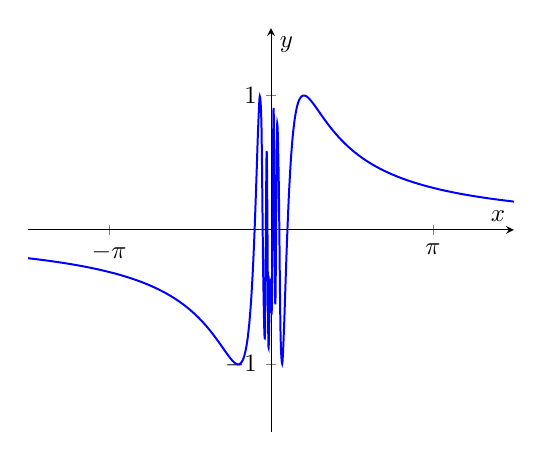
\begin{tikzpicture}[scale=0.9]
        \begin{axis}[
            xmin=-1.5 * pi,
            xmax=1.5 * pi,
            xtick={-pi, pi},
            xticklabels={\( -\pi \), \( \pi \)},
            xticklabel style={anchor=north},
            ymin=-1.5,
            ymax=1.5,
            axis lines=middle,
            xlabel=\(x\),
            ylabel=\(y\),
            every axis plot/.append style={thick}
        ]
            \addplot[color=blue, samples=300, smooth]{sin(deg(1/x))};
        \end{axis}
    \end{tikzpicture}
    \end{center}
\end{itemize}

\subsection{Continuity at Endpoints}

Consider the graph of a function \( y = f \left( x \right) \).

\begin{center}
    \begin{tikzpicture}[scale=0.9]
        \begin{axis}[
            xmin=-2,
            xmax=2,
            xtick={-1, 1},
            xticklabels={\( a \), \( b \)},
            xticklabel style={anchor=north},
            ymin=-2,
            ymax=2,
            axis lines=middle,
            xlabel=\(x\),
            ylabel=\(y\),
            every axis plot/.append style={thick}
        ]
            \addplot[color=blue, domain=-1:1]{1};
            \addplot[hole, color=blue, fill=bg] coordinates {(-1, 1)};
            \addplot[mark=*, color=blue, fill=blue] coordinates {(1, 1)};
        \end{axis}
    \end{tikzpicture}
\end{center}

We can see that at both \( x = a \) and \( x = b \), the function does not continue. When this happens, we call those points \defterm{endpoints}.

\begin{definition}{continuity at endpoints}
    A function is continuous at some endpoint(s) if
    
    \[ \lim_{x \to a^+} f \left( x \right) = f \left( a \right) \]
    \begin{center}
        \textbf{or}
    \end{center}
    \[ \lim_{x \to b^-} f \left( x \right) = f \left( b \right) \]
    
    where \( a \) represents a left endpoint and \( b \) represents a right endpoint.
\end{definition}

\subsection{Removing Discontinuities}

A common exercise that might be asked of you is to locate and remove a discontinuity in a function by rewriting it as a piece-wise function. Sometimes difficulty will arise in identifying where the discontinuity is, while other times it will be evaluating it. Remember to only remove discontinuities if told to do so.

\begin{example}{removing discontinuities}
    The function \( y = \frac{\sin{x}}{x} \) is defined for all real numbers except for \( x = 0 \). If you were asked to remove the discontinuity at \( x = 0 \), thereby making the function continuous, what value would you put in?
    
    Because continuity requires that the limit and the function value must equal, let us take the limit and see what value we need to have at \( x = 0 \).
    
    \[ \lim_{x \to 0} \dfrac{\sin{x}}{x} = 1 \]
    
    So, in order for us to make the function continuous, we should define it to be equal to \( 1 \) at \( x = 0 \). Now that we have this information, we can write our function. Remember to only ever replace discontinuities with number values and to leave the original function otherwise unchanged.
    
    \[
    f \left( x \right) = \begin{cases}
        \dfrac{\sin{x}}{x}, & x \ne 0 \\
        1, & x = 0
    \end{cases}
    \]
\end{example}

Sometimes you will also be tasked with finding out \textit{where} the removable discontinuity is. Questions like this usually involve factoring. Remember, if there is the same zero term in the numerator and denominator, there will likely be a removable discontinuity at that \( x \) value. Just make sure to show your limit work for arriving at that value.

\begin{example}{locating a discontinuity}
    Take a look at the function
    
    \[ y = \dfrac{x^3 - 7x - 6}{x^2 - 9} \]
    
    Locating a discontinuity for a function like this is a clear exercise in factoring.
    
    \[ y = \dfrac{\left( x^2 + 3x + 2 \right) \left( x - 3 \right)}{\left( x - 3 \right) \left( x + 3 \right)} \]
    
    Here, we can see that there is an \( \left( x - 3 \right) \) term in both the numerator and denominator, leading us to believe that there should be a removable discontinuity at \( x = 3 \). To show our work for this, evaluate the limit as \( x \) approaches \( 3 \).
    
    \[ \lim_{x \to 3} \dfrac{\left( x^2 + 3x + 2 \right) \cancel{\left( x - 3 \right)}}{\cancel{\left( x - 3 \right)} \left( x + 3 \right)} = \dfrac{10}{3} \]
    
    Now, we can rewrite our function to be continuous
    
    \[
    f \left( x \right) = \begin{cases}
        \dfrac{x^3 - 7x - 6}{x^2 - 9}, & x \ne 3 \\
        \dfrac{10}{3}, & x = 3
    \end{cases}
    \]
\end{example}

\section{Maximums, Minimums, and Intermediates}

In this section, we'll be able to identify local and global maximum and minimum values and use them in interpreting graphs.

\subsection{Extreme Values}

\begin{theorem}{Min-Max Theorem/Extreme Value Theorem}
    If \( f \) is continuous at every point of a closed interval \( [a, b] \), then \( f \) takes on both a maximum value \( M \) and a minimum value \( m \) somewhere in that interval, and \( m \le f \left( x \right) \le M \) at every other point \( x \) of the interval.
\end{theorem}

This theorem, although worded in a formal way, is quite intuitive. For some continuous function over an interval, there must be a largest and smallest value somewhere in the interval. This can also be seen with a graph.

\begin{center}
    \begin{tikzpicture}[scale=0.9]
        \begin{axis}[
            xmin=-pi,
            xmax=pi,
            xtick={-3 * pi / 4, -pi/2, pi / 2, 3 * pi / 4},
            xticklabels={\( a \), \( x_1 \), \( x_2 \), \( b \)},
            xticklabel style={anchor=north},
            ymin=-1.5,
            ymax=1.5,
            ytick={-1, 1},
            yticklabels={\( m \), \( M \)},
            yticklabel style={anchor=east},
            axis lines=middle,
            xlabel=\(x\),
            ylabel=\(y\),
            every axis plot/.append style={thick}
        ]
            \addplot[color=blue, domain=-3*pi/4:3*pi/4, smooth, samples=200]{sin(deg(x))};
            \addplot[color=Plum, mark=*] coordinates {(-pi/2, -1)} node[anchor=north]{\( \left( x_1, m \right) \)};
            \addplot[color=Plum, mark=*] coordinates {(pi/2, 1)} node[anchor=south]{\( \left( x_2, M \right) \)};
        \end{axis}
    \end{tikzpicture}
\end{center}

Here we see that, in the interval from \( x = a \) to \( x = b \), there is only one minimum point \( \left( x_1, m \right) \) and only one maximum point \( \left( x_2, M \right) \), with all other values of the function between those two numbers.

\subsection{Absolute and Local Extrema}

In Calculus, we make the distinction between absolute, or global, minimums and maximums as opposed to local, or relative, minimums and maximums.

\begin{definition}{absolute minimum/maximum}
    The \defterm{absolute minimum or maximum} is the \textit{one} lowest or highest point of the graph, respectively. If there is a discontinuity at the point in which there should be an absolute extremum, the absolute extremum does not exist.
\end{definition}

\begin{definition}{local minimum/maximum}
    \defterm{Local minimums and maximums} are, as the name would suggest, locally minimal or maximal relative to their surroundings. There can be multiple local extrema in a graph, and local extrema can also be global extrema.
\end{definition}

\begin{example}{absolute and local extrema}
    Let us take a look at some graph \( y = g \left( x \right) \).

    \begin{center}
        \begin{tikzpicture}[scale=0.9]
            \begin{axis}[
                xmin=-0.1,
                xmax=4,
                xticklabels={,,},
                yticklabels={,,},
                ymin=-0.1,
                ymax=2,
                axis lines=middle,
                xlabel=\(x\),
                ylabel=\(y\),
                every axis plot/.append style={thick}
            ]
                \addplot[color=blue, samples=200, domain=-0.1:3.25]{0.25 * sin(3 * deg(x)) + 0.5 * x};
                \addplot[hole, color=purple, fill=examplebg] coordinates {(2.86123643, 1.615700076)} node[color=black, anchor=south]{\( M_a \)};
                \addplot[mark=*, color=blue, fill=blue] coordinates {(0, 0)} node[color=black, anchor=south west]{\( m_a \)};
                \addplot[mark=*, color=blue, fill=blue] coordinates {(0.7668413277, 0.569759662)} node[color=black, anchor=south]{\( M_l \)};
                \addplot[mark=*, color=blue, fill=blue] coordinates {(1.327553775, 0.4774378892)} node[color=black, anchor=south]{\( m_l \)};
                \addplot[mark=*, color=blue, fill=blue] coordinates {(2.86123643, 1.3)};
            \end{axis}
        \end{tikzpicture}
    \end{center}
    
    In this graph, we have an absolute minimum at \( m_a \), and a local minimum at \( m_l \). We also have a local maximum \( M_l \). However, take close note to the discontinuity where the maximum \( M_a \) \textit{should} be. Despite the function being continuous at every other point, because there is no defined largest value, \textbf{the absolute maximum does not exist}.
\end{example}

\subsection{Bounded Functions}

\begin{definition}{bounded function}
    A function \( f \left( x \right) \) is said to be \defterm{bounded above} a value \( c \) if all values of the function are less than or equal to that value \( c \). Similarly, a function \( f \left( x \right) \) is said to be \defterm{bounded below} a value \( c \) if all values of the function are greater than or equal to that value \( c \).
    
    \vspace{0.2cm}
    
    A function is considered \defterm{bounded} when it has \textbf{both} a lower and upper bound.
\end{definition}

\begin{example}{bounded function}
    The function \( y = \sin{x} \) is bounded above by \( y = 1 \) (or any value greater than \( 1 \) as well) and bounded below by \( y = -1 \). From this, we can see that the function \( y = \sin{x} \) is a bounded function.
\end{example}

One use case for this is being able to find an inequality that you can use with the Sandwich Theorem to evaluate a limit. Although this will not be used too often, it is helpful to know the terminology. 

\subsection{Intermediate Values}

\begin{theorem}{Intermediate Value Theorem}
    A function \( y = f \left( x \right) \) that is continuous on a closed interval \( [a, b] \) takes on every value between \( f \left( a \right) \) and \( f \left( b \right) \).
\end{theorem}

This theorem, when deconstructed, is also quite intuitive. If a function does not have any discontinuities, then it must pass through all the values in a given interval. You might also see this phrased as: you can associate at least one \( x \) value in the interval \( [a, b] \) to any \( y \) value in the interval \( [f \left( a \right), f \left( b \right)] \).

\begin{center}
    \begin{tikzpicture}[scale=0.9]
        \begin{axis}[
            xmin=-0.1,
            xmax=2,
            xtick={0.25, pi/4 + 0.25, 0.25 + pi/2},
            xticklabels={\( a \), \( c \), \( b \)},
            xticklabel style={anchor=north},
            ymin=-0.1,
            ymax=1.5,
            ytick={0.479848847066, 0.64352079242, 1.1707354924},
            yticklabels={\( f \left( a \right) \), \( f \left( c \right) \), \( f \left( b \right) \)},
            yticklabel style={anchor=east},
            axis lines=middle,
            xlabel=\(x\),
            ylabel=\(y\),
            every axis plot/.append style={thick}
        ]
            \addplot[color=blue, samples=200, smooth, domain=0.25:0.25 + pi/2]{pow(sin(deg(3 / 2 * x - 7 / 8)), 2) + 1 / 4};
            \addplot[color=blue, mark=*] coordinates {(0.25, 0.479848847066)};
            \addplot[color=blue, mark=*] coordinates {(pi/4 + 0.25, 0.64352079242)};
            \addplot[color=blue, mark=*] coordinates {(0.25 + pi/2, 1.1707354924)};
            
            \addplot[color=gray, dashed] coordinates {(0, 0.479848847066) (0.25, 0.479848847066) (0.25, 0)};
            \addplot[color=blue, dashed] coordinates {(0, 0.64352079242) (pi/4 + 0.25, 0.64352079242) (pi/4 + 0.25, 0)};
            \addplot[color=gray, dashed] coordinates {(0, 1.1707354924) (pi/2 + 0.25, 1.1707354924) (pi/2 + 0.25, 0)};
        \end{axis}
    \end{tikzpicture}
\end{center}

One common exercise involving the IVT is to prove that there exists a \( 0 \) of a function in some interval.

\begin{example}{using the IVT}
    Given the equation
    
    \[ f \left( x \right) = x^3 + x^2 - 4x - 3 \]
    
    Prove that there is a \( 0 \) of the function somewhere in the interval \( [1, 2] \).
    
    \vspace{0.5cm}
    
    Plugging in the bounds of the interval into the function, we get
    
    \begin{align*}
        f \left( 1 \right) &= -5, \\
        f \left( 2 \right) &= 1
    \end{align*}
    
    Combining our knowledge of all polynomial functions being continuous, we can understand that the function should pass through the \( x \)-axis somewhere in the given interval. A full explanation utilizing the theorem would look something like:
    
    \vspace{0.3cm}
    
    "Because \( f \left( x \right) \) is continuous between \( [1, 2] \) it takes on every value between \( -5 \) and \( 1 \). Because \( -5 \le 0 \le 1 \), the function must equal \( y = 0 \) at some point between \( x = 1 \) and \( x = 2 \) by the Intermediate Value Theorem."
\end{example}
